\let\negmedspace\undefined
\let\negthickspace\undefined
\documentclass[journal]{IEEEtran}
\usepackage[a5paper, margin=10mm, onecolumn]{geometry}
%\usepackage{lmodern} % Ensure lmodern is loaded for pdflatex
\usepackage{tfrupee} % Include tfrupee package

\setlength{\headheight}{1cm} % Set the height of the header box
\setlength{\headsep}{0mm}     % Set the distance between the header box and the top of the text

\usepackage{gvv-book}
\usepackage{gvv}
\usepackage{cite}
\usepackage{amsmath,amssymb,amsfonts,amsthm}
\usepackage{algorithmic}
\usepackage{graphicx}
\usepackage{textcomp}
\usepackage{xcolor}
\usepackage{txfonts}
\usepackage{listings}
\usepackage{enumitem}
\usepackage{mathtools}
\usepackage{gensymb}
\usepackage{comment}
\usepackage[breaklinks=true]{hyperref}
\usepackage{tkz-euclide} 
\usepackage{listings}
\usepackage{gvv}                                        
\def\inputGnumericTable{}                                 
\usepackage[latin1]{inputenc}                                
\usepackage{color}                                            
\usepackage{array}                                            
\usepackage{longtable}                                       
\usepackage{calc}                                             
\usepackage{multirow}                                         
\usepackage{hhline}                                           
\usepackage{ifthen}                                           
\usepackage{lscape}
\usepackage{circuitikz}
\tikzstyle{block} = [rectangle, draw, fill=blue!20, 
    text width=4em, text centered, rounded corners, minimum height=3em]
\tikzstyle{sum} = [draw, fill=blue!10, circle, minimum size=1cm, node distance=1.5cm]
\tikzstyle{input} = [coordinate]
\tikzstyle{output} = [coordinate]


\begin{document}

\bibliographystyle{IEEEtran}
\vspace{3cm}

\title{2.10.77}
\author{EE25BTECH11049 - Sai Krishna Bakki}
 \maketitle
% \newpage
% \bigskip
{\let\newpage\relax\maketitle}

\renewcommand{\thefigure}{\theenumi}
\renewcommand{\thetable}{\theenumi}
\setlength{\intextsep}{10pt} % Space between text and floats


\numberwithin{equation}{enumi}
\numberwithin{figure}{enumi}
\renewcommand{\thetable}{\theenumi}

\textbf{Question}:\\
The points $(-a, -b)$, $(0, 0)$, $(a, b)$ and $(a^2, ab)$ are
\begin{enumerate}
\item Collinear
\item Vertices of a parallelogram
\item Vertices of a rectangle
\item None of these
\end{enumerate}
\solution \\
Given:
\begin{align}
\vec{A}=\myvec{-a\\-b},\vec{B}=\myvec{0\\0},\vec{C}=\myvec{a\\b},\vec{D}=\myvec{a^2\\ab}
\end{align}
Condition for the points to be vertices of a parallelogram is \\
\begin{align}
    \vec{B}-\vec{A}=\vec{C}-\vec{D}\\
    \vec{B}-\vec{A}=\myvec{a\\b},\vec{C}-\vec{D}=\myvec{a-a^2\\b-ab}
\end{align}
But
\begin{align}
\vec{B}-\vec{A} \neq \vec{C}-\vec{D}
\end{align} 
If
$\vec{B}-\vec{A} \neq \vec{C}-\vec{D}$ then the points cannot be vertices of a rectangle too because every rectangle is a specific type of parallelogram.

Condition for the points to be collinear is
\begin{align}
    \text{rank}\myvec{\vec{B} - \vec{A} & &\vec{C} - \vec{D}} = 1
\end{align}
\begin{align}
    \text{rank}\myvec{a & a-a^2\\b & b-ab}
\end{align}
\begin{align}
	\myvec{a &  a-a^2\\ b & b-ab} \xleftrightarrow[]{R_2 \rightarrow {\frac{-b}{a}R_1 + R_2}} \myvec{a & a-a^2 \\ 0 & 0}  
\end{align}
The number of non zero rows in the row reduced matrix (also known as {\em echelon form}) is defined as the rank.\\
For the above matrix, Rank is one.\\
Therefore, we can conclude that four points are collinear.
\newpage
 \begin{figure}
    \centering
    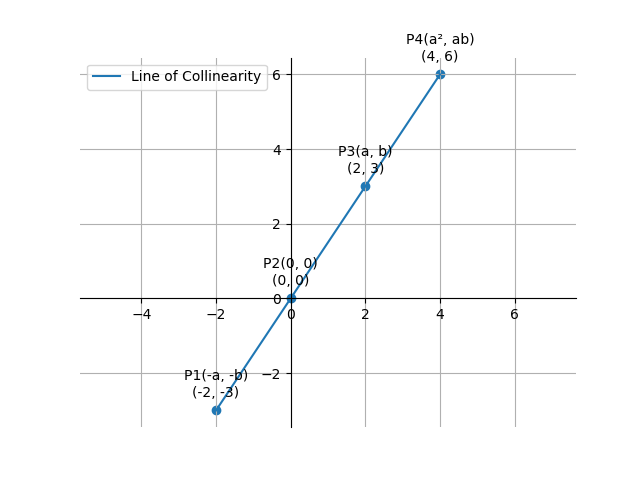
\includegraphics[width=0.9\columnwidth]{figs/Figure_1.png}
    \label{fig:placeholder}
    \caption{}
\end{figure}
\end{document}
